\section{Experiment 2}
\label{sec:exp2}
Experiment 2, similarly to experiment 1, trains and evaluates ANNs for the task to classify images of fruits and vegetables. Experiment 2, however, considers 131 labels, making the classification task more challenging. The goal of experiment 2, as in experiment 1, is to try different network types in order to find the best configuration, i.e., the configuration with the lowest zero-one loss, and to see if the best configuration for experiment 1, still holds for experiment 2.

\subsection{Setup}
The setup is very similar to experiment 1. The experiment is run on the same machine, using networks build by the \texttt{models.py} script.

\textbf{Dataset.} The same dataset of images is used, however all the 90380 images and all the 131 labels are considered this time. For this reason, datasets are managed by a different script, \texttt{dataset\_2.py}, and they are stored in a different folder. The script works in the same way as \texttt{dataset\_1.py}.

\textbf{Models and execution}. The models used are the same type and shapes used in experiment 1. Indeed the script \texttt{models.py} is reused. The execution of the experiment is managed by the script \texttt{experiment\_2.py} which works in the same way as \texttt{experiment\_1.py}, except for the dataset used and the folder to store the results.

\subsection{Results}
The results collected are summarized in table \ref{table:exp2}. The table contains the list of 150 ANNs trained and evaluated, with their parameters, i.e., depth, width and type, the number of epochs they were trained for and the zero-one loss achieved on the testing set.
\input exp2_table

Figure \ref{fig:e2_loss_epochs} shows the zero-one loss and the number of epochs of each ANNs, differentiating the DNNs from the CNNs.
\begin{figure}
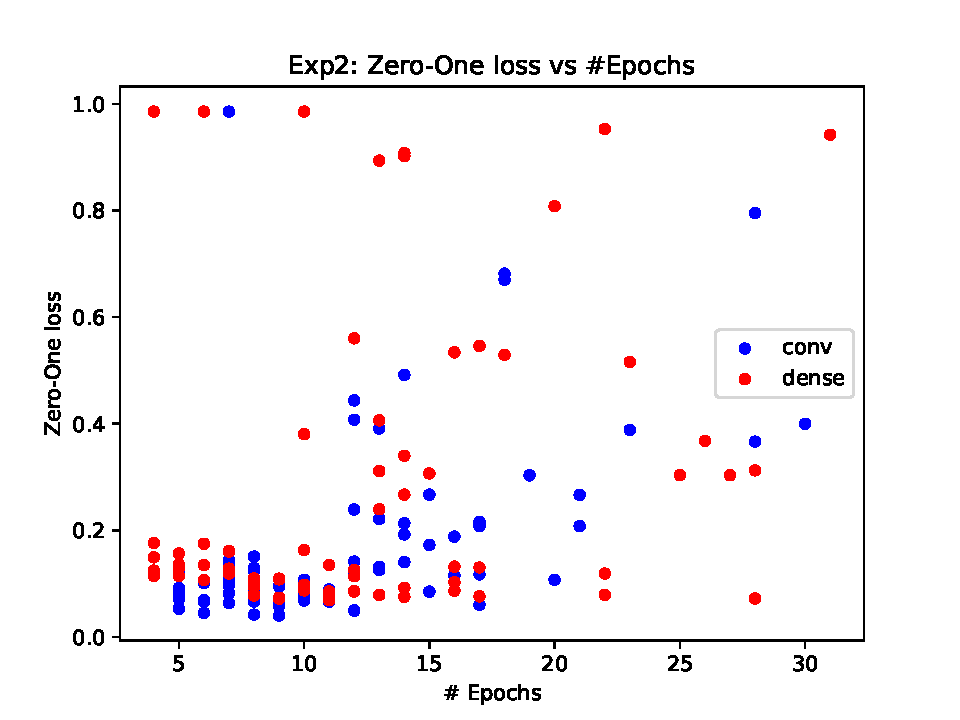
\includegraphics[width=\textwidth]{e2_loss_epochs}
\caption{Experiment 1: zero-one loss vs epochs}\label{fig:e2_loss_epochs}
\end{figure}
The average loss achieved by DNNs is 0.29, whereas the average loss achieved by CNNs is 0.19. The minimum loss achieved by DNNs is 0.07, whereas the minimum loss achieved by CNNs is 0.04. The best configuration for DNNs is: depth 1, width 160 and input images of 10x10 pixels. This network was trained for 11 epochs. The best configuration for CNNs is: depth 2, width 24 and input images of 30x30 pixels. This network was trained for 9 epochs. The best DNN uses 10x10 images both in experiment 1 and in experiment 2. All other parameters are different between best networks of both experiments. The best DNN for experiment 1 has 0.12 loss in experiment 2. The best CNN for experiment 1 has 0.10 loss in experiment 2.

Figure \ref{fig:e2_50_loss_width} shows the zero-one loss achieved on images of size 50x50 pixels by ANNs of different depth and width, of type DNN and CNN respectively. The figures show that deeper and wider networks achieve a lower zero-one loss. Note that small differences in loss do not represent overfitting because loss is computed on the testing set, i.e., on data that was not used during training.
\begin{figure}
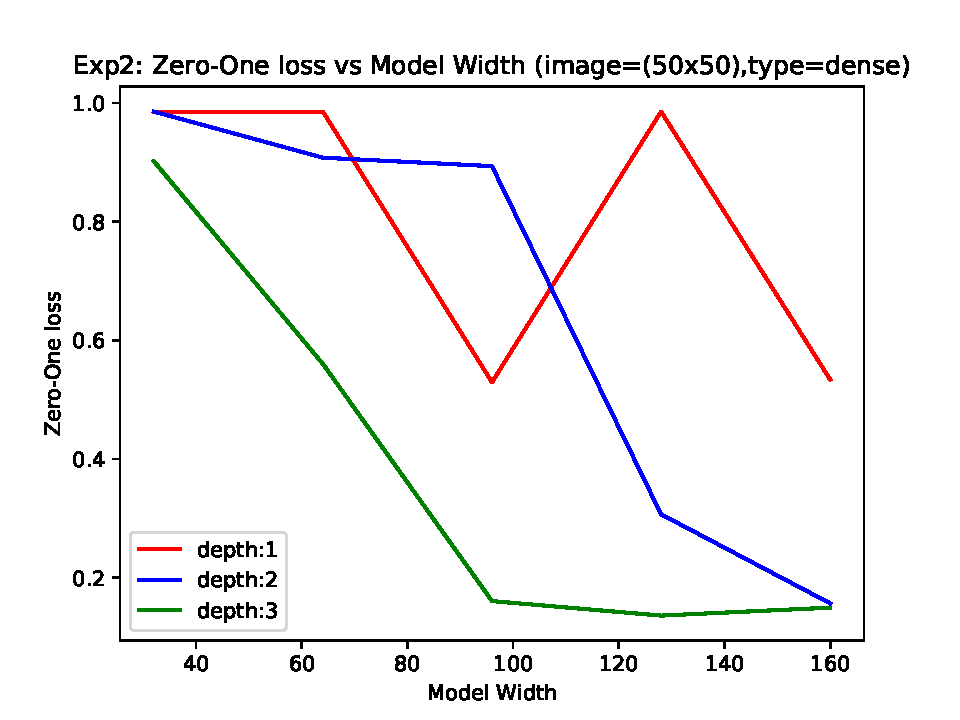
\includegraphics[width=\textwidth]{e2_50_dense_loss_width}
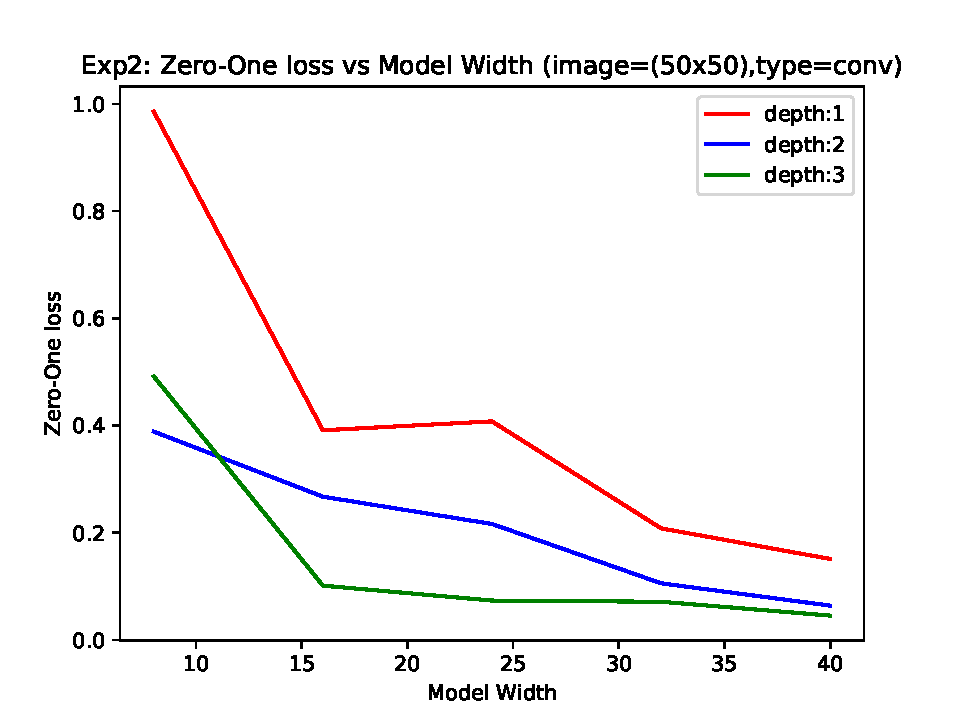
\includegraphics[width=\textwidth]{e2_50_conv_loss_width}
\caption{Experiment 2: zero-one loss vs ANN size}\label{fig:e2_50_loss_width}
\end{figure}

Figure \ref{fig:e2_30_history_accuracy_image_size} shows the accuracy history of all ANNs computed during the training phase on the validation. The figure shows that a lot of networks tend to achieve a accuracy higher than 80\% after just 1 epoch. This is slower than in experiment 1, as shown in figure \ref{fig:e1_30_history_accuracy_image_size}. Furthermore CNNs appear to converge faster than DNNs, with a few exceptions. The slowest network to converge is a DNN, which appears not able to be trained at all.
\begin{figure}
\includegraphics[width=\textwidth]{e2_30_history_accuracy_image_size}
\caption{Experiment 1: accuracy history during training}\label{fig:e2_30_history_accuracy_image_size}
\end{figure}

Results can be reproduced by following the steps highlighted in section\ref{sec:repro}.
